%%%%%%%%%%%%%%%%%%%%%%%%%%%%%%%%%%%%%%%%%%%%%%%%%%%%%%%%%%%%%%%%%%%%%%%%%%%%%%%%%%%%%%%%%%%%%%%%%%%
\documentclass[10pt, a4paper]{article}
%%%%%%%%%%%%%%%%%%%%%%%%%%%%%%%%%%%%%%%%%%%%%%%%%%%%%%%%%%%%%%%%%%%%%%%%%%%%%%%%%%%%%%%%%%%%%%%%%%%

%--------------------------------------------------------------------------------------------------
% Dimensions :
%--------------------------------------------------------------------------------------------------

\setlength{\textheight}{25.9cm}
\setlength{\textwidth}{16cm}

\setlength{\topmargin}{-21mm}
\setlength{\oddsidemargin}{0mm}
\setlength{\evensidemargin}{0mm}

% \setlength{\columnsep}{20mm}

\setlength{\fboxsep}{1mm}
\setlength{\unitlength}{1mm}

%--------------------------------------------------------------------------------------------------
% Packages :
%--------------------------------------------------------------------------------------------------

\usepackage{latexsym}
\usepackage{graphicx}
\usepackage{pifont}
\usepackage{color}
\usepackage{amsmath}
\usepackage{amssymb}

\usepackage[french]{babel}    % pour franciser le document

%\usepackage[latin1]{inputenc} % pour utiliser les caracteres accentues du claviers
\usepackage[utf8]{inputenc}

%--------------------------------------------------------------------------------------------------
% Divers :
%--------------------------------------------------------------------------------------------------

% Couleurs :
\definecolor{blanc}{rgb}{1.0, 1.0, 1.0}
\definecolor{gris}{rgb}{0.8, 0.8, 0.8}
\definecolor{grisfonce}{rgb}{0.7, 0.7, 0.7}
\definecolor{vert}{rgb}{0.2, 0.6, 0.2}
\definecolor{rouge}{rgb}{0.8, 0.2, 0.0}
%\definecolor{bleu}{rgb}{0.0, 0.5, 0.7}
\definecolor{bleu}{rgb}{0.2, 0.4, 0.6}
\definecolor{experimental}{rgb}{0.6, 0.7, 0.4}
\definecolor{numerique}{rgb}{0.8, 0.2, 0.0}
\definecolor{theorique}{rgb}{0.0, 0.5, 0.7}

% Chemin d'accès des figures :
\graphicspath{{../FIGURES/}{Figures/}{Abstract/}}

\usepackage{cancel}
% Style des vecteurs : fleche ou gras ?

%\newcommand{\myvec}[1]{\boldsymbol{#1}}
\newcommand{\myvec}[1]{\vec{#1}}

\newcommand{\mytensor}[1]{\accentset{\Rightarrow}{#1}} % needs \usepackage{accents}

%---------------------------
% Operateurs differentiels :
%---------------------------

\newcommand{\divergence}{\mbox{\rm div}\,}

\newcommand{\gradient}{\myvec{\mbox{\rm gra}}\mbox{\rm d}}
% \newcommand{\gradient}{\mathbf{grad}\,}
% \newcommand{\ggradient}{\stackrel{\Rightarrow}{\mbox{gra}}\!\!\!\,\mbox{d}\,}
\newcommand{\ggradient}{\accentset{\Rightarrow}{\mbox{\rm gra}}\mbox{\rm d}\!}

%\renewcommand{\dot}[1]{\accentset{\hbox{\huge .}}{#1}}
\newcommand{\mydot}[1]{\accentset{\centerdot}{#1}}

\newcommand{\rot}{\vec{\mbox{\rm ro}}\mbox{\rm t}\,}
%\newcommand{\rot}{\mathbf{rot}\,}

% \newcommand{\vnabla}{\vec{\nabla}}
\newcommand{\vnabla}{\boldsymbol{\nabla}}

% Fonctions speciales:

\newcommand{\besselj}[1]{\mbox{J}_{#1}}
\newcommand{\besselk}[1]{\mbox{K}_{#1}}
\newcommand{\bessely}[1]{\mbox{Y}_{#1}}
\newcommand{\besseli}[1]{\mbox{I}_{#1}}

% Vecteurs, tenseurs et torseurs:

\newcommand{\ex}{\mathbf{e}_{x}}
\newcommand{\ey}{\mathbf{e}_{y}}
\newcommand{\ez}{\mathbf{e}_{z}}

\newcommand{\er}{\mathbf{e}_{r}}
\newcommand{\erho}{\mathbf{e}_{\rho}}
\newcommand{\ephi}{\mathbf{e}_{\varphi}}
\newcommand{\etheta}{\mathbf{e}_{\theta}}

%\newcommand{\tensor}[1]{\stackrel{\Rightarrow}{#1}}
\newcommand{\tensor}[1]{\mbox{\sl \textbf{#1}}}
\newcommand{\torseur}[4]{
   \!\!\!\! \left . \begin{array}{c} \\ \\ _#1 \end{array} \!\!\!
   \right \{ \!\!\!
   \begin{array}{#4} #2 \\ \\ #3 \end{array}}

% Integrales multiples:

\newcommand{\odblint}[1]{\int\!\!\!\!\!\int_{#1} \hskip -7mm \bigcirc \;}
\newcommand{\dblint}{\int\!\!\!\!\!\int}
\newcommand{\tplint}{\int\!\!\!\!\!\int\!\!\!\!\!\int}

% Fractions:

\renewcommand{\dfrac}[2]{\displaystyle \frac{#1}{#2}}

% Derivees ordinaires et partielles:

\newcommand{\dpdt}[1]{\dfrac{\partial #1}{\partial t}}
\newcommand{\dpdx}[1]{\dfrac{\partial #1}{\partial x}}
\newcommand{\dpdy}[1]{\dfrac{\partial #1}{\partial y}}
\newcommand{\dpdz}[1]{\dfrac{\partial #1}{\partial z}}

\newcommand{\ddpdt}[1]{\dfrac{\partial^2 #1}{\partial t^2}}
\newcommand{\ddpdx}[1]{\dfrac{\partial^2 #1}{\partial x^2}}
\newcommand{\ddpdy}[1]{\dfrac{\partial^2 #1}{\partial y^2}}
\newcommand{\ddpdz}[1]{\dfrac{\partial^2 #1}{\partial z^2}}

\newcommand{\dpdr}[1]{\dfrac{\partial #1}{\partial r}}
\newcommand{\dpdrho}[1]{\dfrac{\partial #1}{\partial \rho}}
\newcommand{\dpdphi}[1]{\dfrac{\partial #1}{\partial \varphi}}
\newcommand{\dpdtheta}[1]{\dfrac{\partial #1}{\partial \theta}}

\newcommand{\ddpdr}[1]{\dfrac{\partial^2 #1}{\partial r^2}}
\newcommand{\ddpdrho}[1]{\dfrac{\partial^2 #1}{\partial \rho^2}}
\newcommand{\ddpdphi}[1]{\dfrac{\partial^2 #1}{\partial \varphi^2}}
\newcommand{\ddpdtheta}[1]{\dfrac{\partial ^2#1}{\partial \theta^2}}

\newcommand{\ddt}[1]{\dfrac{d #1}{dt}}
\newcommand{\ddx}[1]{\dfrac{d #1}{dx}}
\newcommand{\ddy}[1]{\dfrac{d #1}{dy}}
\newcommand{\ddz}[1]{\dfrac{d #1}{dz}}
\newcommand{\ddr}[1]{\dfrac{d #1}{dr}}

\newcommand{\ddtref}[2]{\dfrac{d #1}{dt}_{\! | #2 }}
\newcommand{\dpdtref}[3]{\dfrac{\partial #1}{\partial #2}_{\! | #3 }}

% Misc:

\newcommand{\mycaption}[1]{\caption{\sl #1}}

\newcommand{\ligne}[1]{\hrule height #1\linethickness \hfill}

\newcommand{\thickline}[2]{\linethickness{#1} \line(1, 0){#2}}

\newcommand{\myline}{\noindent\underline{\hspace{\textwidth}}}
\newcommand{\mysection}[1]{\vskip 0.5cm \section{#1}\vskip -1.4cm 
   \myline \vskip 0.4cm \myline \bigskip}

\newcommand{\etal}{\textit{et al.}}

\newcommand{\varray}[1]{\renewcommand{\arraystretch}{#1}}

\newcommand{\puissance}[1]{^{\mbox{\footnotesize #1}}}
\newcommand{\indice}[1]{_{\mbox{\footnotesize #1}}}

%---------------------------------------------------------------------
% New environments:
%---------------------------------------------------------------------

\newcounter{MyEnumCounter}
\newcounter{MySaveCounter}
\newenvironment{MyEnum}{%
  \begin{list}{\arabic{MyEnumCounter}.}{\usecounter{MyEnumCounter}%
  \setcounter{MyEnumCounter}{\value{MySaveCounter}}}
  }{%
  \setcounter{MySaveCounter}{\value{MyEnumCounter}}\end{list}%
}
\newcommand{\MyEnumReset}{\setcounter{MySaveCounter}{0}}

\newenvironment{deuxcols}{\begin{tabular}{lr} \hspace*{-9.7mm}}{\end{tabular}}

\newenvironment{dem}{\noindent %
   \begin{tabular}{||l} \textsl{D\'emonstration :} \\ % 
   \begin{minipage}{15.5cm} \footnotesize} %
   {\end{minipage}\end{tabular}}

\newenvironment{abst}{\begin{quotation}\sl}{\end{quotation}}

\newenvironment{eqnbox}{\begin{equation}\begin{array}{|c|}  \hline \\ 
   \displaystyle}{\\ \\ \hline \end{array} \end{equation}}

\newcommand{\myprime}{\ \!'}

% JFM symbols:

\DeclareMathSymbol{\varGamma}{\mathord}{letters}{"00}
\DeclareMathSymbol{\varDelta}{\mathord}{letters}{"01}
\DeclareMathSymbol{\varTheta}{\mathord}{letters}{"02}
\DeclareMathSymbol{\varLambda}{\mathord}{letters}{"03}
\DeclareMathSymbol{\varXi}{\mathord}{letters}{"04}
\DeclareMathSymbol{\varPi}{\mathord}{letters}{"05}
\DeclareMathSymbol{\varSigma}{\mathord}{letters}{"06}
\DeclareMathSymbol{\varUpsilon}{\mathord}{letters}{"07}
\DeclareMathSymbol{\varPhi}{\mathord}{letters}{"08}
\DeclareMathSymbol{\varPsi}{\mathord}{letters}{"09}
\DeclareMathSymbol{\varOmega}{\mathord}{letters}{"0A}

% ---------------------------------------------------------------------
% MISC SYMBOLS :
% ---------------------------------------------------------------------

\font\SY=msam10 
\def\carreblanc{\hbox{\SY \char'3}}
\def\carrenoir{\hbox{\SY \char'4}}
\def\diamblanc{\hbox{\SY \char'6}}
\def\diamnoir{\hbox{\SY \char'7}}
\def\triblancright{\hbox{\SY \char'102}}
\def\triblancleft{\hbox{\SY \char'103}}
\def\triblancup{\hbox{\SY \char'115}}
\def\triblancdown{\hbox{\SY \char'117}}
\def\trinoirright{\hbox{\SY \char'111}}
\def\trinoirleft{\hbox{\SY \char'112}}
\def\trinoirup{\hbox{\SY \char'116}}
\def\trinoirdown{\hbox{\SY \char'110}}
\def\rondblanc{\hbox{\scriptsize $\bigcirc$}}
\def\rondnoir{\hbox{\LARGE $\bullet$}}

\font\BB=msbm10 scaled 1095
\def\setr{\hbox{\BB R}}
\def\setc{\hbox{\BB C}}
\def\setn{\hbox{\BB N}}
\def\setz{\hbox{\BB Z}}

% Pour enlever la numerotation des pages de la table des matieres:

%%%% debut macro, a placer dans preambule %%%%
\makeatletter
\def\addcontentsline@toc#1#2#3{%
   \addtocontents{#1}{\protect\thispagestyle{empty}}%
   \addtocontents{#1}{\protect\contentsline{#2}{#3}{\thepage}}}
\def\addcontentsline#1#2#3{%
  \expandafter\@ifundefined{addcontentsline@#1}%
  {\addtocontents{#1}{\protect\contentsline{#2}{#3}{\thepage}}}
  {\csname addcontentsline@#1\endcsname{#1}{#2}{#3}}}
\makeatother
%%%% fin macro %%%%

\newcommand{\titre}[1]{ %
  \medskip \noindent \underline{\makebox[\textwidth][l]{\textbf{#1}\textcolor{white}{pl}}}}% \\}

\newcommand{\sstitre}[1]{ %
  \bigskip \centerline{\textbf{#1}} \smallskip}

\def\draft{\overfullrule 5pt} % The \draft command marks the overful boxes

\def\indentlist{\list%
        {}{\labelwidth 0pt \leftmargin 3\labelsep}}
\let\endindentlist\endlist \relax

\def\datelist{\list%
        {}{\settowidth\labelwidth{[2001/02 :]}
        \leftmargin\labelwidth
        \advance\leftmargin\labelsep}
}
\let\enddatelist\endlist \relax

\def\longuelist{\list%
        {}{\settowidth\labelwidth{[Etablissement :]}
        \leftmargin\labelwidth
        \advance\leftmargin\labelsep}
}
\let\endlonguelist\endlist \relax

\def\shortlist{\list%
        {}{\settowidth\labelwidth{$\bullet$}
        \leftmargin\labelwidth
        \advance\leftmargin\labelsep}
}
\let\endshortlist\endlist \relax



\renewcommand{\thickline}[2]{\linethickness{#1} \line(1, 0){#2}}
\renewcommand{\mycaption}[1]{\caption{\sl #1}}
\renewcommand{\myvec}[1]{\vec{#1}}

% \pagestyle{empty}

\graphicspath{{Figures/}} % chemin d'acces au repertoire des figures (par ex.)


%%%%%%%%%%%%%%%%%%%%%%%%%%%%%%%%%%%%%%%%%%%%%%%%%%%%%%%%%%%%%%%%%%%%%%%%%%%%%%%%%%%%%%%%%%%%%%%%%%%
\begin{document}
%%%%%%%%%%%%%%%%%%%%%%%%%%%%%%%%%%%%%%%%%%%%%%%%%%%%%%%%%%%%%%%%%%%%%%%%%%%%%%%%%%%%%%%%%%%%%%%%%%%

\begin{center}

  \textsc{Université Toulouse 3 -- Paul Sabatier \hfill Année universitaire 2015-2016}
  
  \textsc{Mécanique des fluides \hfill L3 Mécanique}
  
  \vspace{0mm}
  
  \begin{center}
    \thickline{0.4mm}{160}
    \\ \vspace{3mm}
  \textbf{\large Exercice complémentaire 2 : 
  								premier problème de Stokes\footnote{Ce problème est aussi appelé \textsl{problème de Rayleigh}.}}
    \\ %\vspace{1mm}
    \thickline{0.4mm}{160}
  \end{center}

%  \vspace{0mm}
  
\end{center}

%==================================================================================================
\section{Position du problème}
%==================================================================================================

On s'intéresse au phénomène de diffusion de la quantité de mouvement dans un milieu fluide visqueux
semi-infini, initialement au repos et limité en $x=0$ par une paroi qui est mise en mouvement à vitesse 
constante $U_1$ à partir de $t=0$ (fig.~\ref{fig:entrainement}).
Les portions de fluide en contact avec la paroi sont entraînées verticalement à la vitesse $U_1$ à cause
de la condition d'adhérence, et les frottements visqueux conduisent les couches voisines à se mettre
progressivement en mouvement vers le haut.
Le profil de vitesse verticale $v(x, t)$ évolue alors au cours du temps suivant une loi typique de
diffusion instationnaire dont la dérivation est l'objet de cet exercice.

Ce phénomène a été modélisé et mis en équation en cours. 
L'application du principe de conservation de la quantité de mouvement 
(c'est-à-dire du principe fondamental de la dynamique) pour un volume élémentaire de fluide
et le choix d'une loi de comportement de type fluide newtonien conduisent à l'équation suivante pour la vitesse verticale
du fluide, en l'absence de la pesanteur et pour une pression supposée uniforme :
\begin{equation}
	\dpdt{v} = \nu \, \ddpdx{v}
	\label{eq:diffusion}
\end{equation}
où $\nu$ désigne la viscosité cinématique du fluide (m$^2$/s).
A cette équation d'évolution s'ajoutent la condition limite $v(x=0, t) = U_1$ pour $t > 0$ 
et la condition initiale $v(x, t=0) = 0$ pour $x>0$.

\begin{figure}[tbh]
  \begin{center}
    \begin{picture}(160, 72)(0, -35)
    		% Particules :
 			\put(0, 0){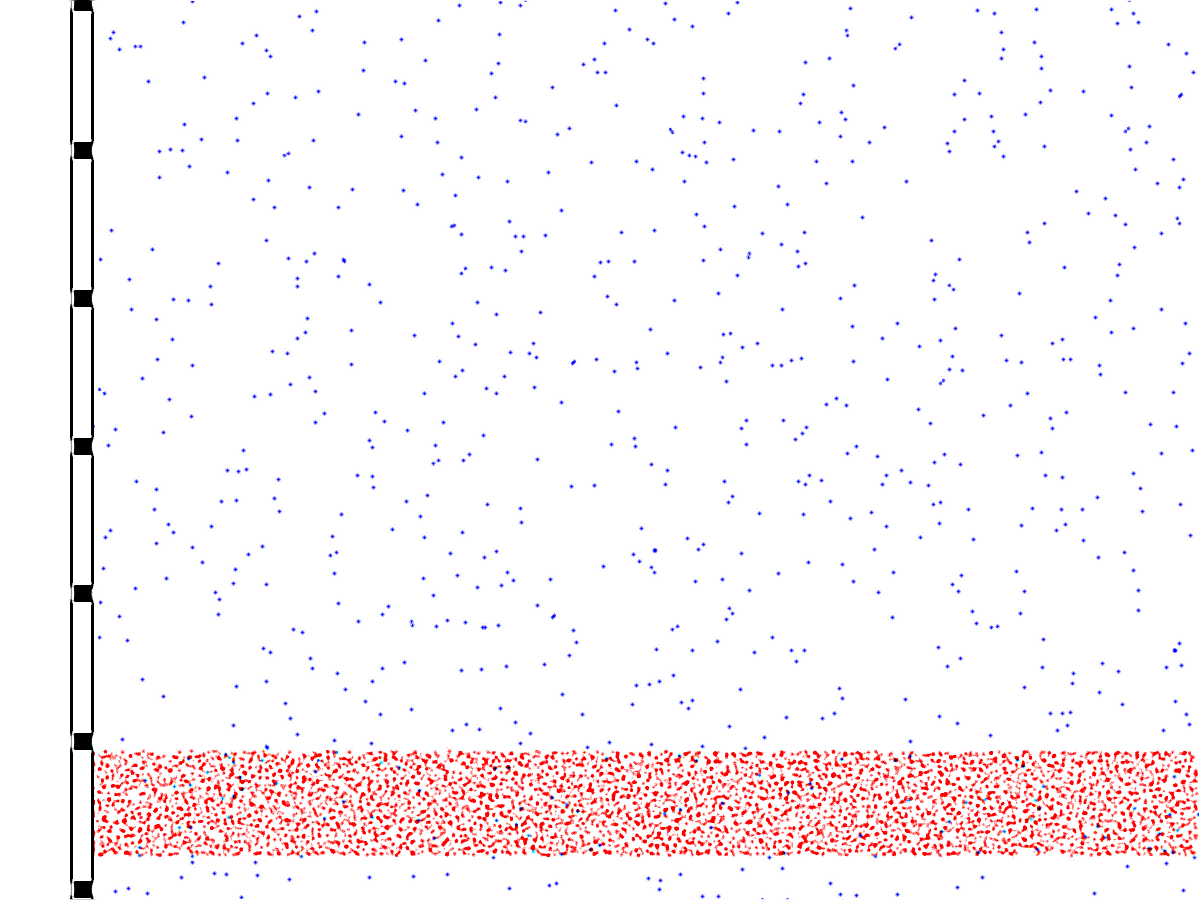
\includegraphics[width=40mm]{momentum_diffusion_particles0_sharp.pdf}}
			\put(2.7, -0.5){\color{bleu}\linethickness{1mm}\line(0, 1){31}}
			\put(25, 7){\vector(1, 0){8}} \put(33, 6.5){\footnotesize \colorbox{white}{$x$}}
			\put(25, 7){\vector(0, 1){8}} \put(23.5, 17){\footnotesize \colorbox{white}{$y$}}
    		\put(20, 30){\footnotesize $t=0^+$}
    		\put(1.5, 10){\vector(0, 1){10}}
    		\put(-1.5, 22){\footnotesize $U_1$}
    		\put(10, 22){\footnotesize $U_0=0$}
 			\put(40, 0){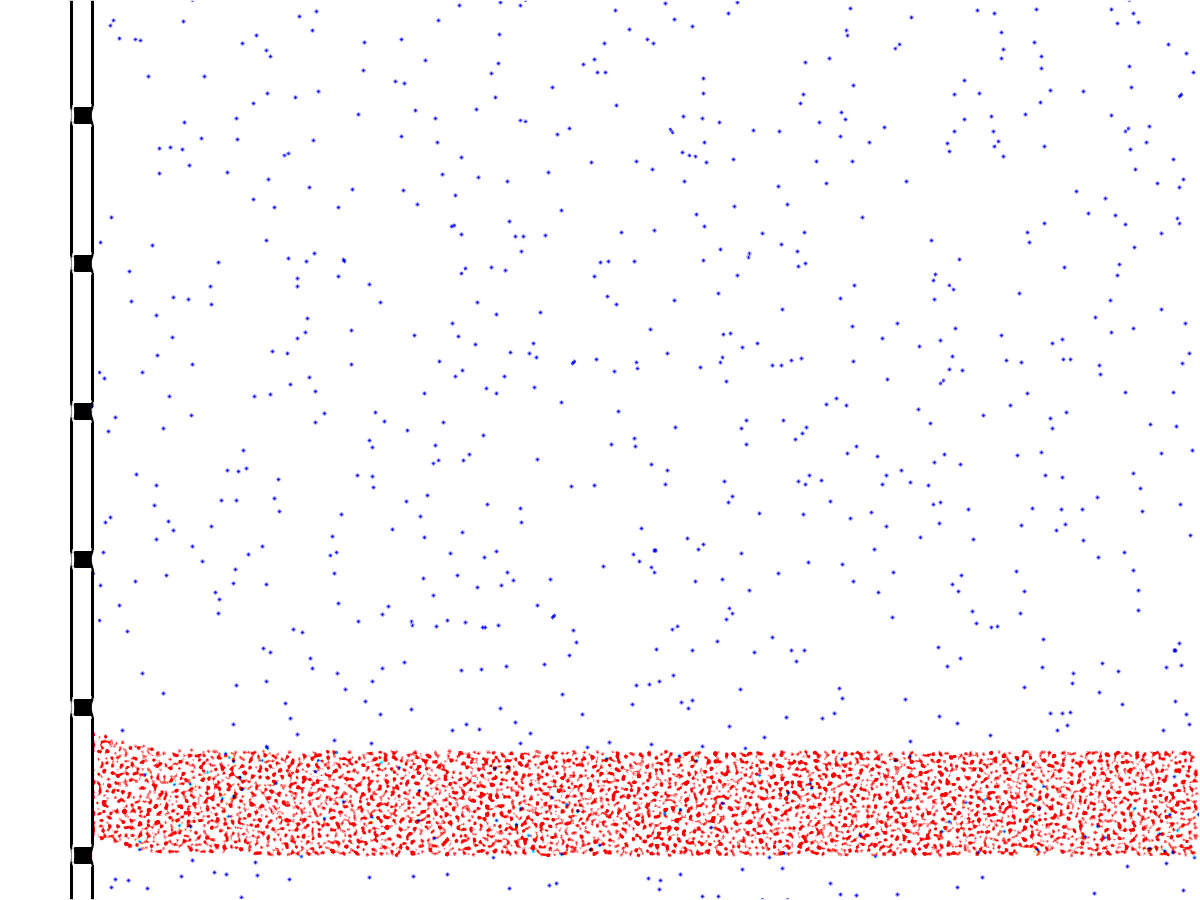
\includegraphics[width=40mm]{momentum_diffusion_particles4_sharp.png}}
			\put(42.7, -0.5){\color{bleu}\linethickness{1mm}\line(0, 1){31}}
			\put(43.1, 1.5){\color{rouge}\linethickness{0.2mm}\vector(1, 0){3}}
    		\put(45, -1.5){\footnotesize \color{rouge} $\delta(t_1)$}
    		\put(60, 30){\footnotesize $t=t_1$}
    		\put(41.5, 10){\vector(0, 1){10}}
 			\put(80, 0){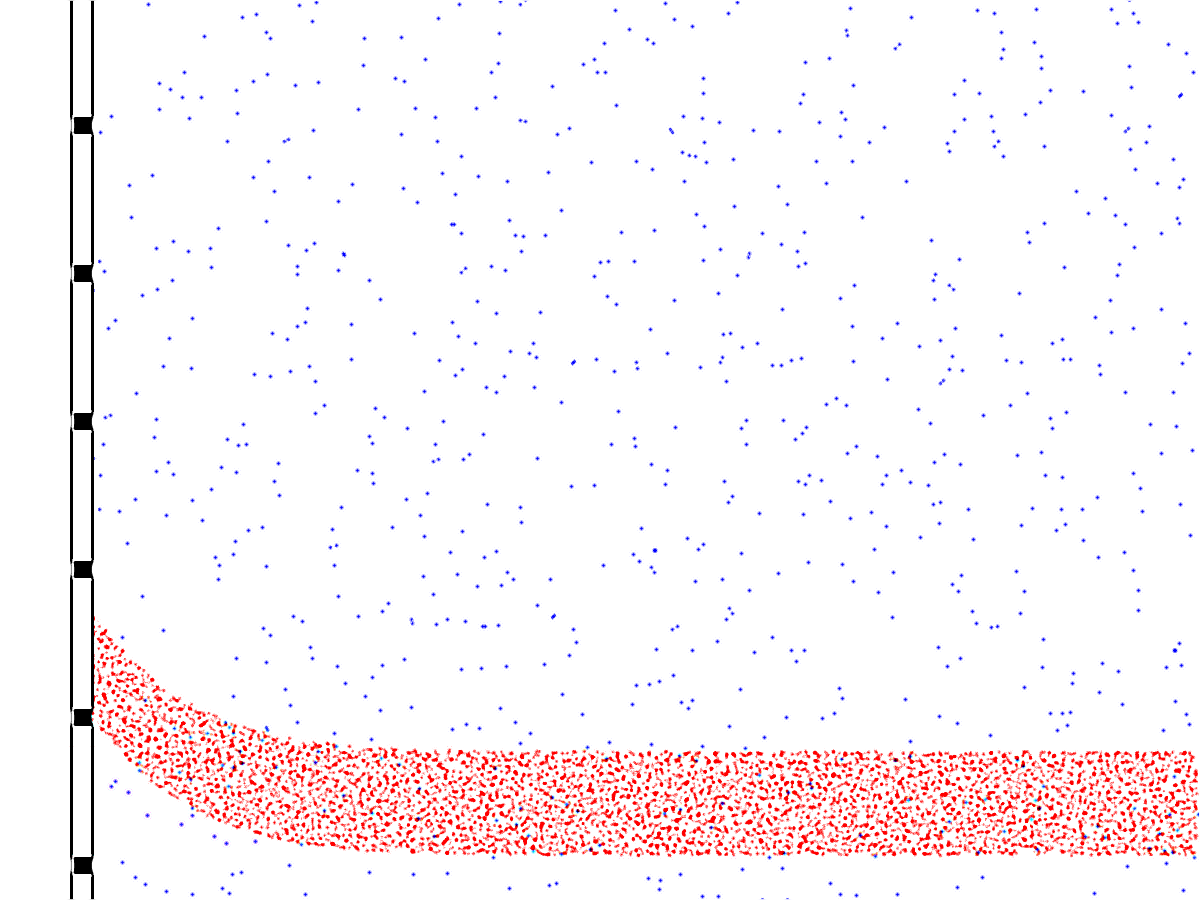
\includegraphics[width=40mm]{momentum_diffusion_particles6_sharp.png}}
			\put(82.7, -0.5){\color{bleu}\linethickness{1mm}\line(0, 1){31}}
			\put(83.1, 1.5){\color{rouge}\linethickness{0.2mm}\vector(1, 0){7}}
    		\put(100, 30){\footnotesize $t=t_2$}
    		\put(81.5, 10){\vector(0, 1){10}}
    		\put(90, -1.5){\footnotesize \color{rouge} $\delta(t_2)$}
 			\put(120, 0){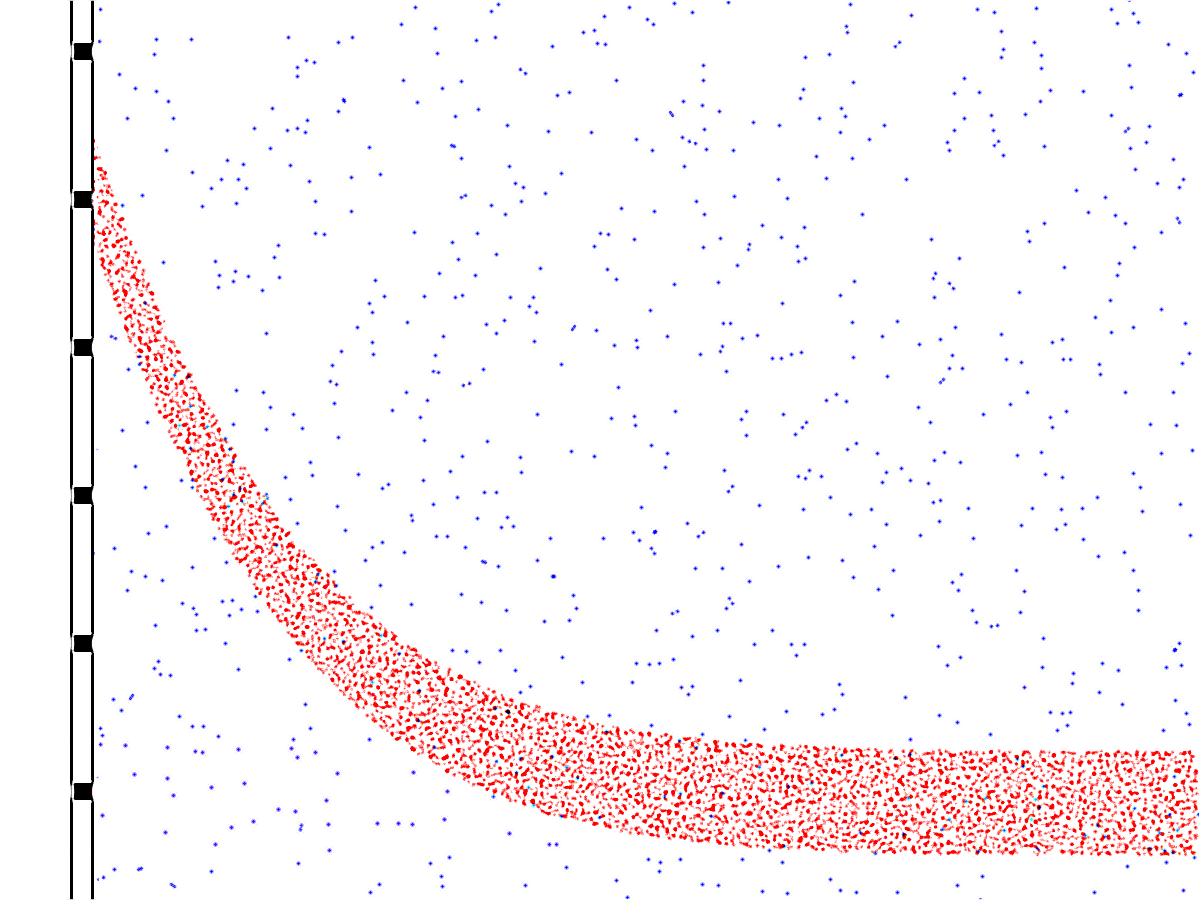
\includegraphics[width=40mm]{momentum_diffusion_particles8_sharp.png}}
			\put(122.7, -0.5){\color{bleu}\linethickness{1mm}\line(0, 1){31}}
			\put(123.1, 1.5){\color{rouge}\linethickness{0.2mm}\vector(1, 0){20}}
    		\put(140, 30){\footnotesize $t=t_3$}
    		\put(121.5, 10){\vector(0, 1){10}}
    		\put(143, -1.5){\footnotesize \color{rouge} $\delta(t_3)$}
			% Profils :
 			\put(  2, -35){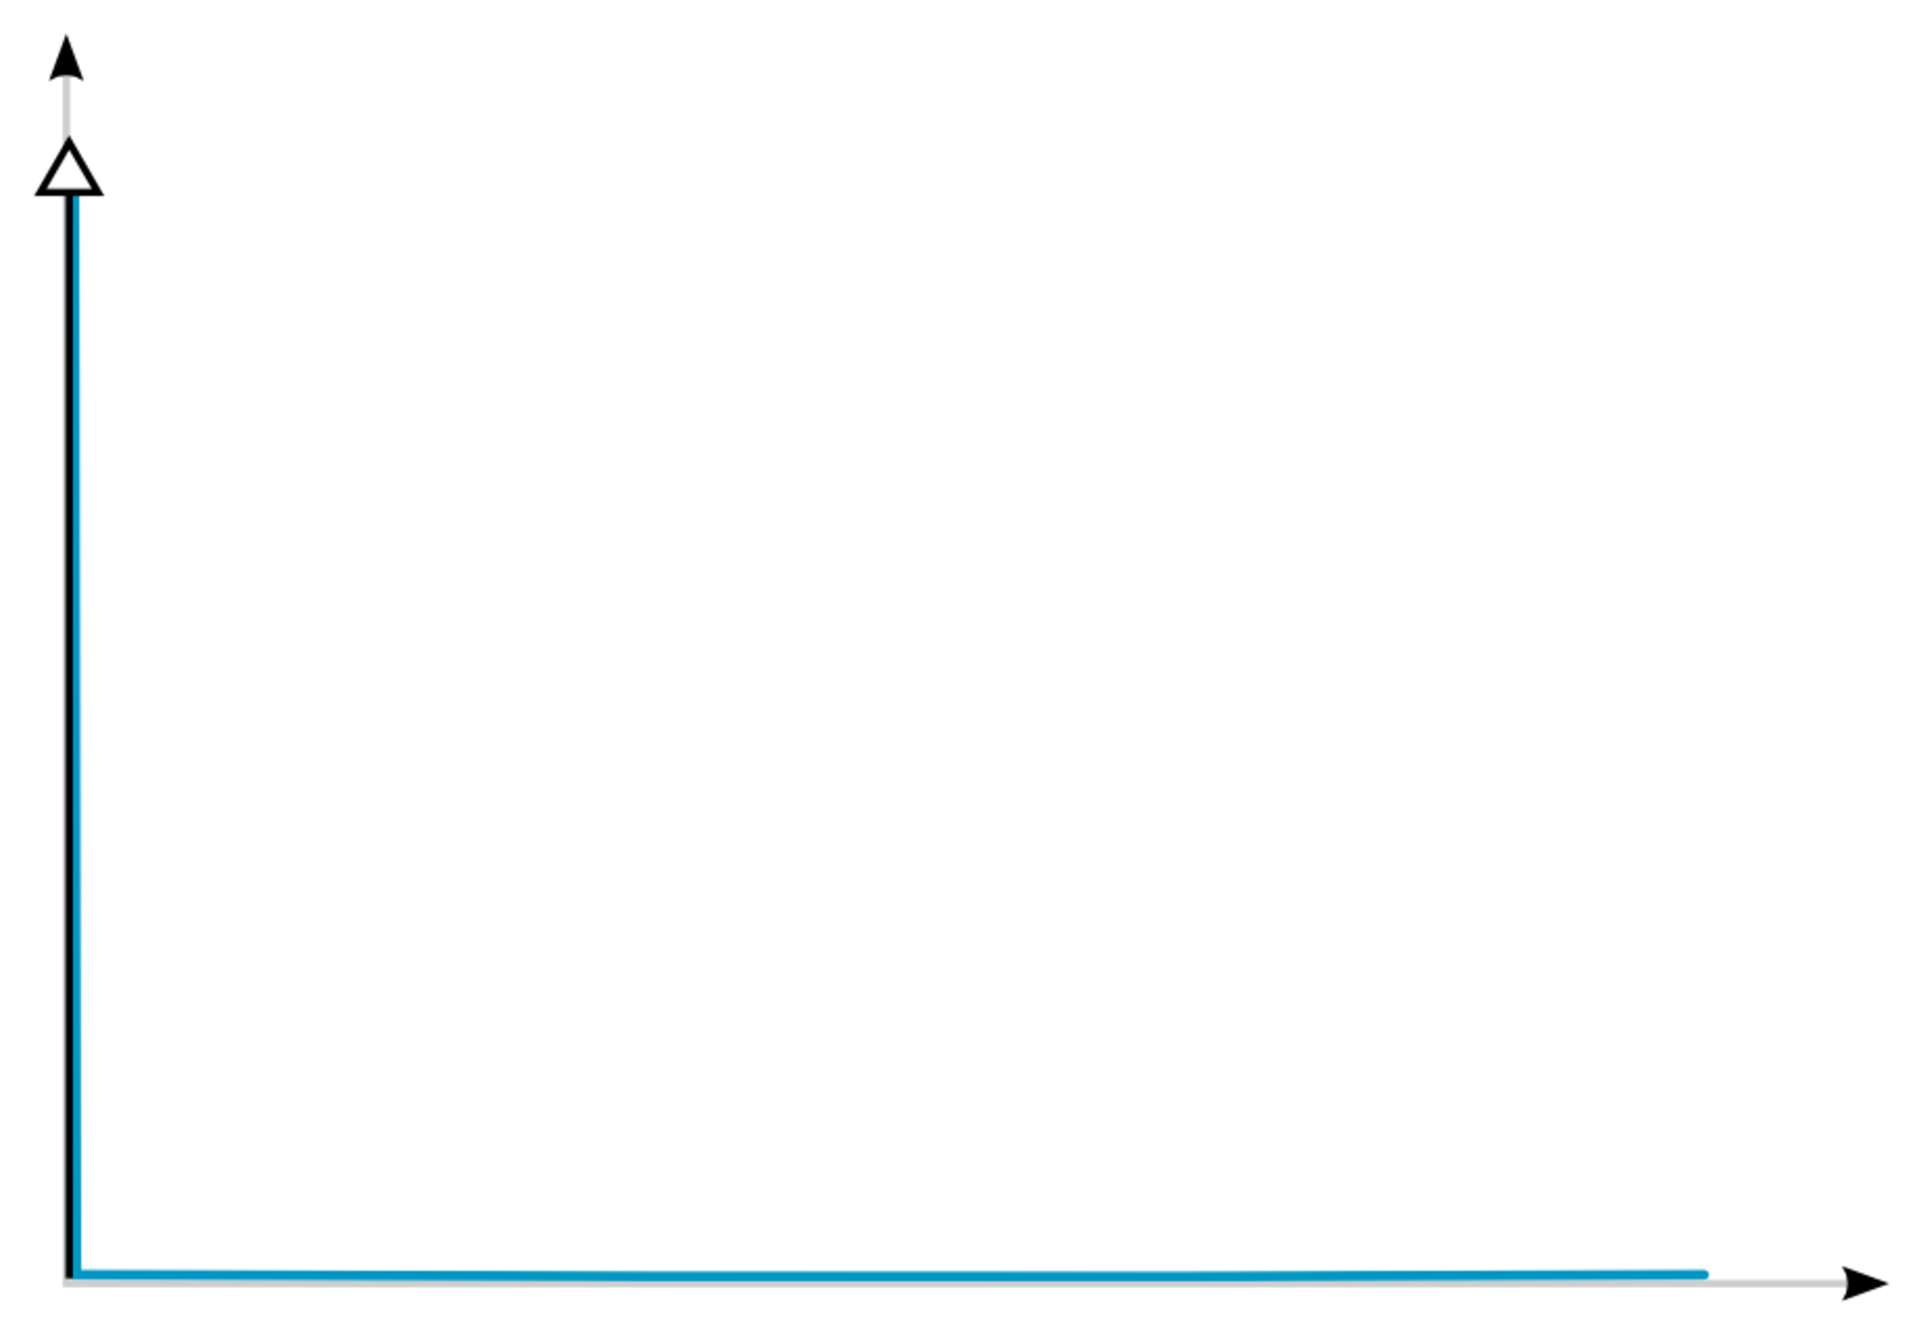
\includegraphics[width=39mm]{momentum_diffusion_profile0.pdf}}
			\put(-1.5, -12){\footnotesize $U_1$}
			\put(  3, -37){\footnotesize $0$}
			\put( 37, -37){\footnotesize $x$}
			\put( 10, -30){\footnotesize \color{bleu} $v(x, 0)$}
 			\put( 42, -35){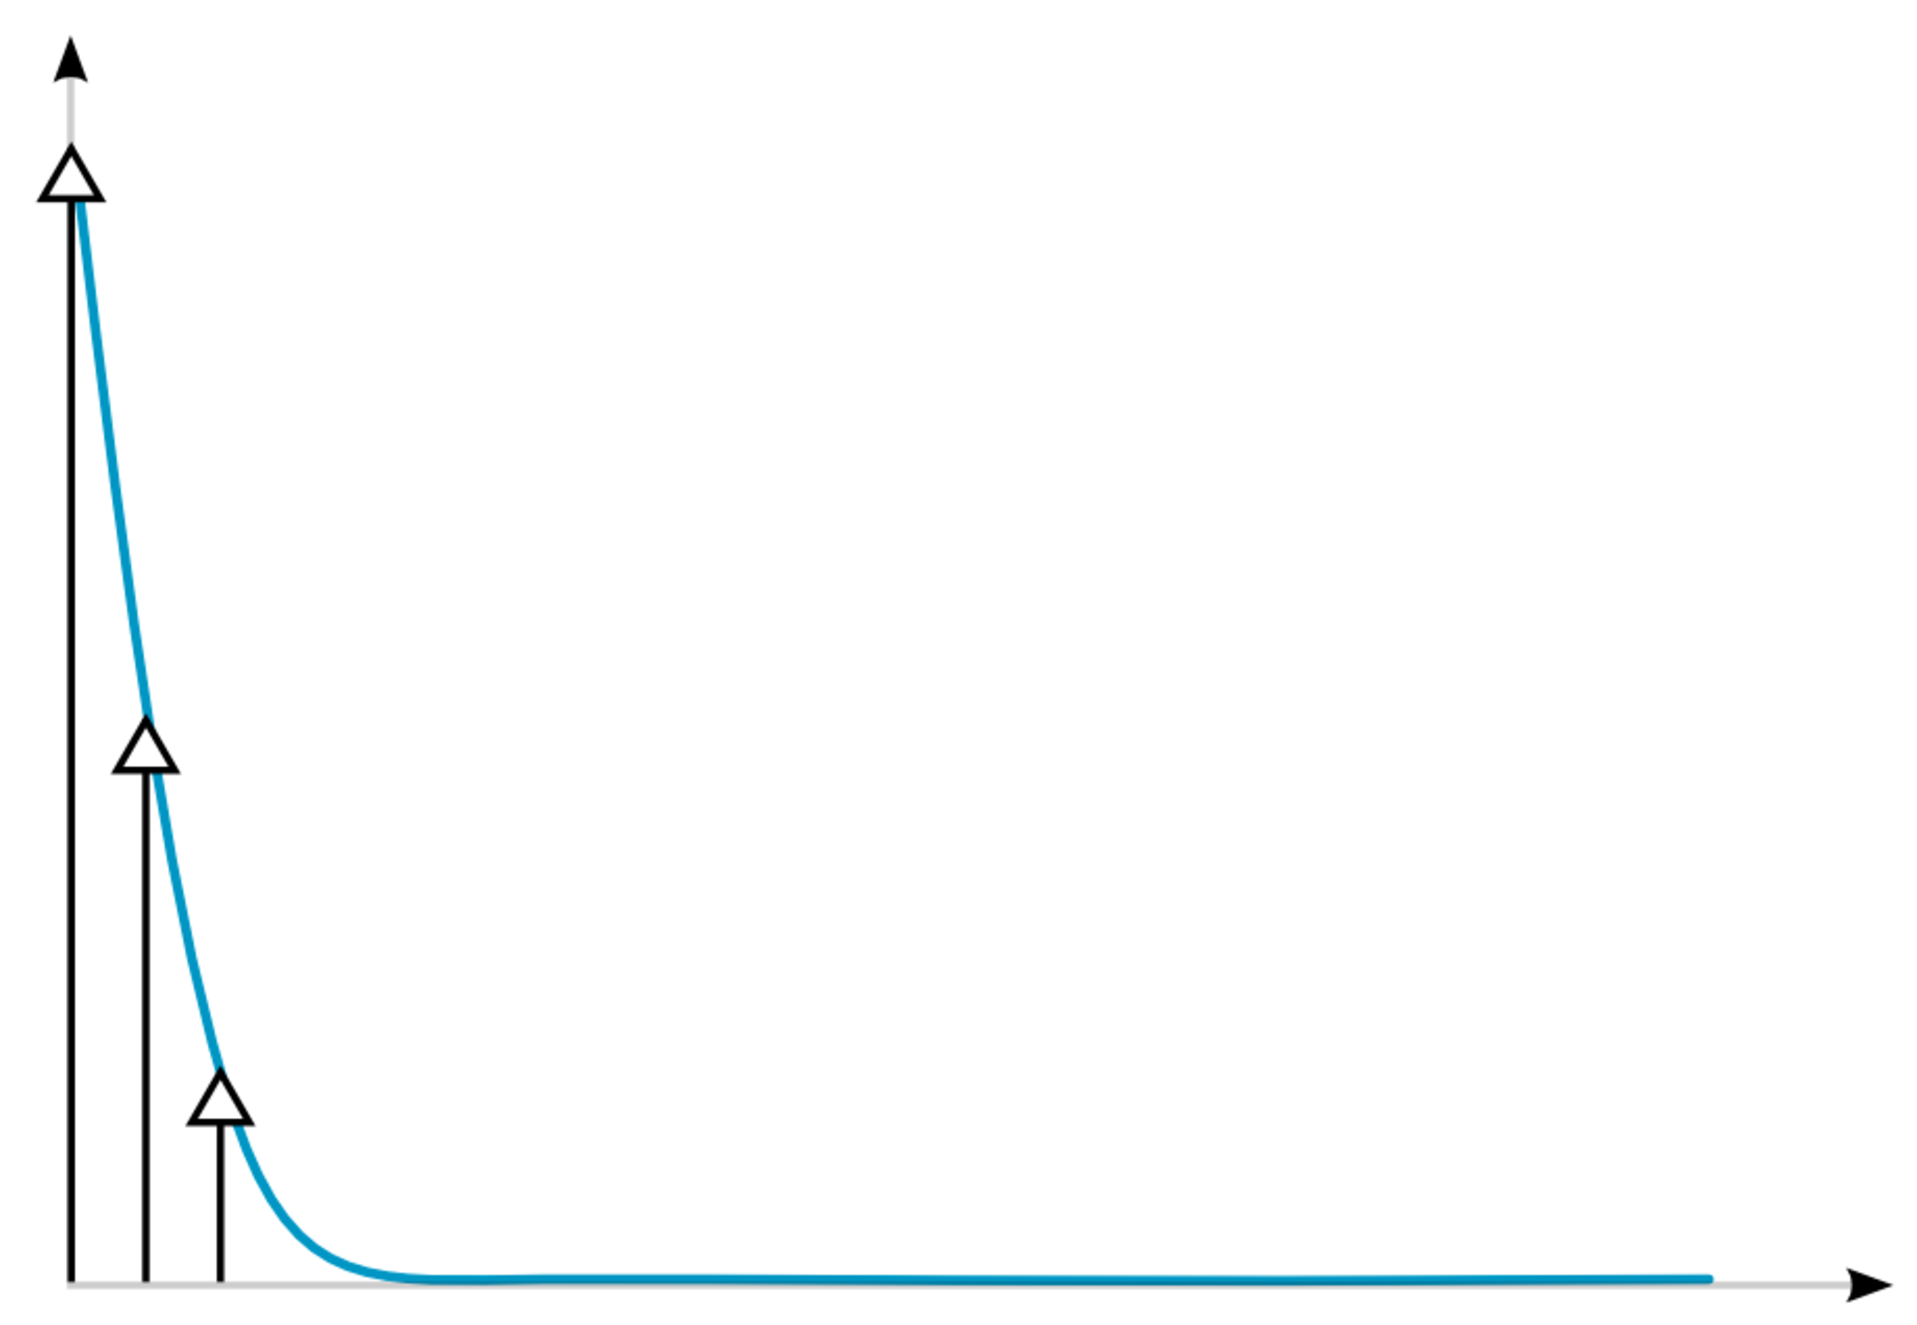
\includegraphics[width=39mm]{momentum_diffusion_profile4.pdf}}
			\put(38.5, -12){\footnotesize $U_1$}
			\put( 55, -30){\footnotesize \color{bleu} $v(x, t_1)$}
 			\put( 82, -35){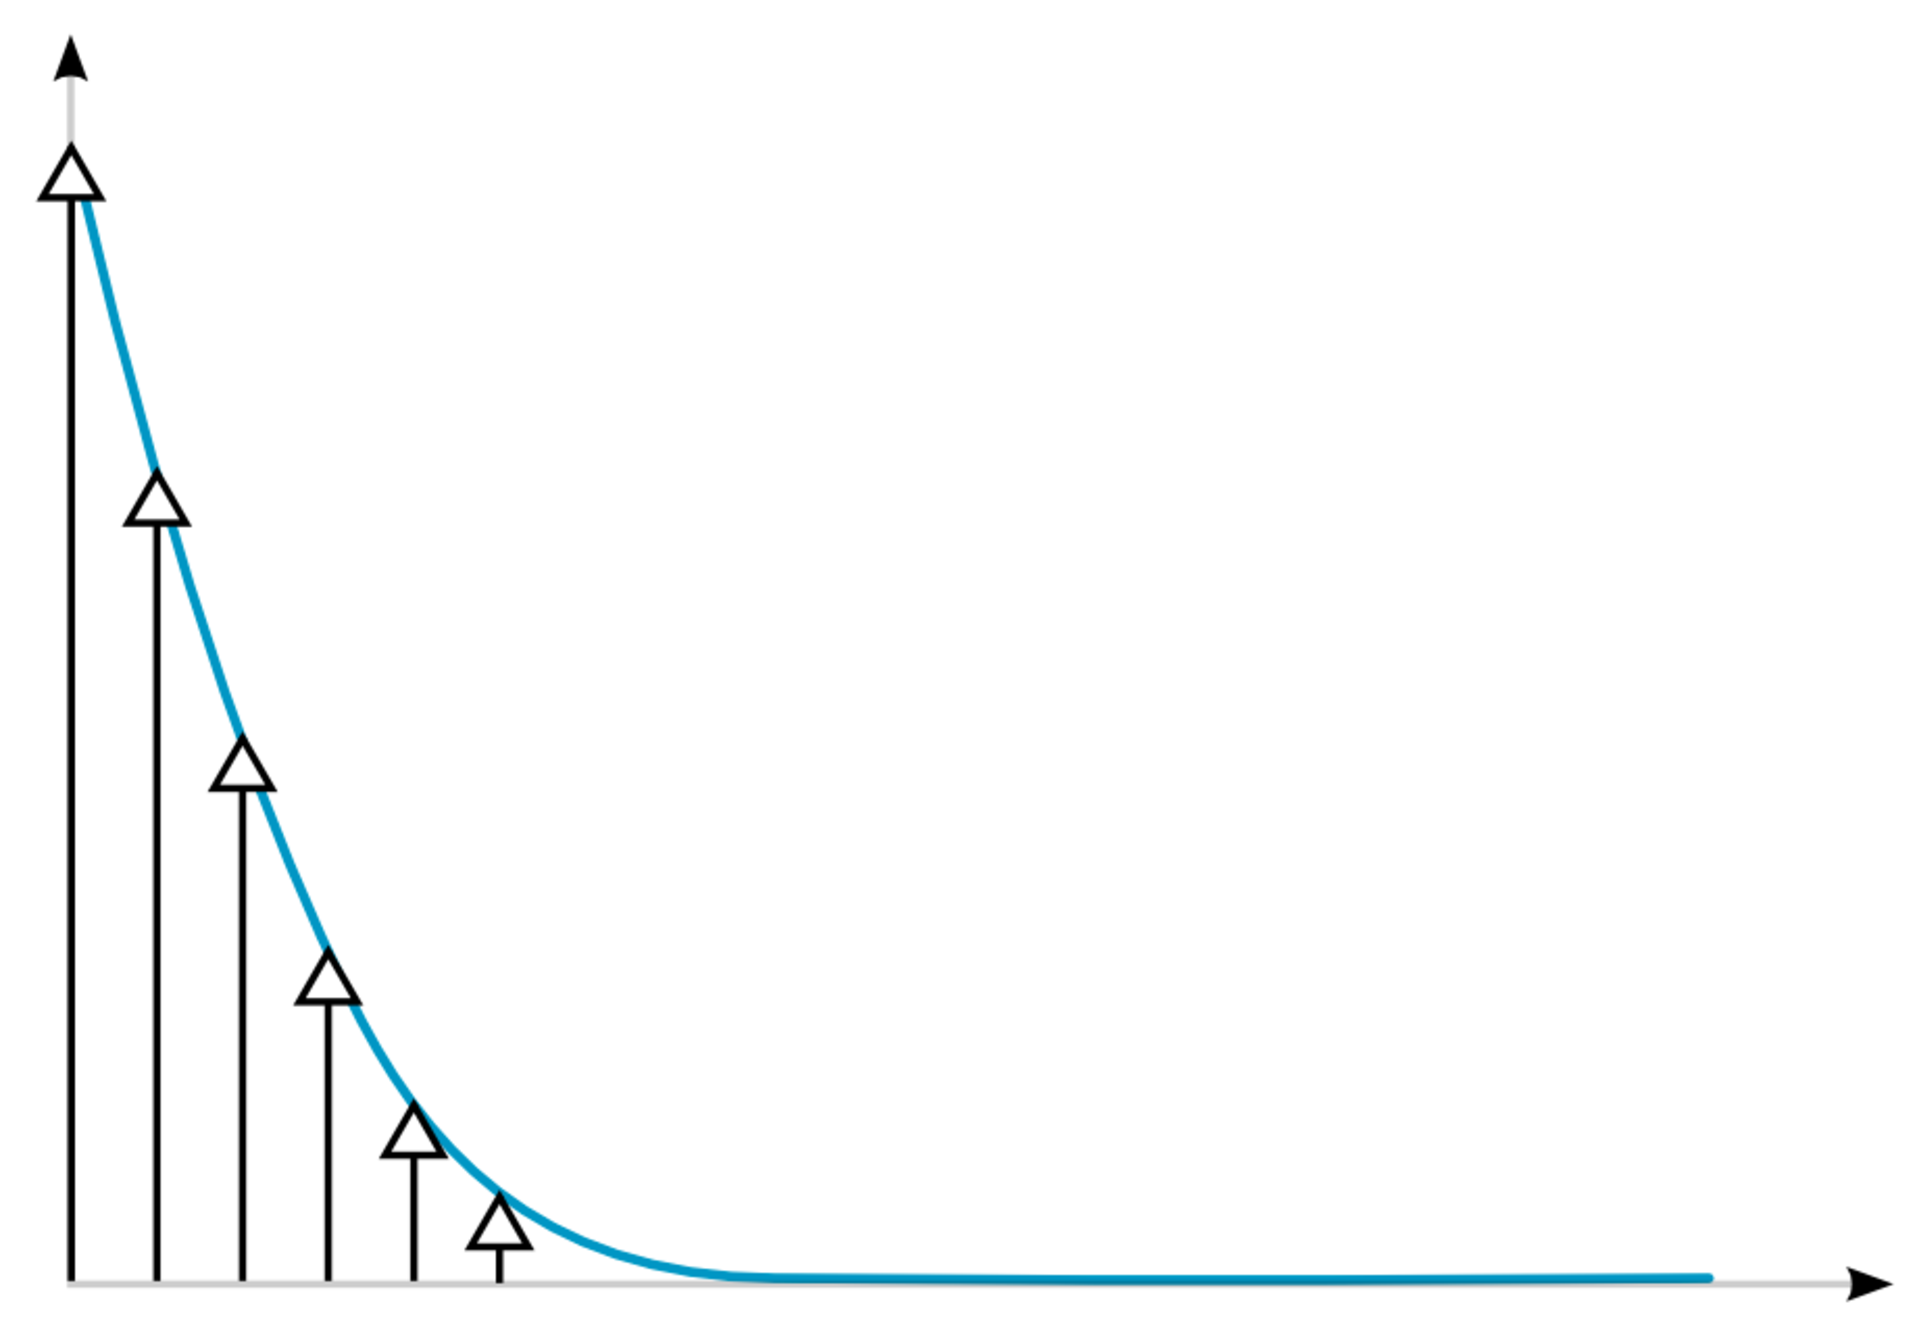
\includegraphics[width=39mm]{momentum_diffusion_profile6.pdf}}
			\put(78.5, -12){\footnotesize $U_1$}
			\put(100, -30){\footnotesize \color{bleu} $v(x, t_2)$}
 			\put(122, -35){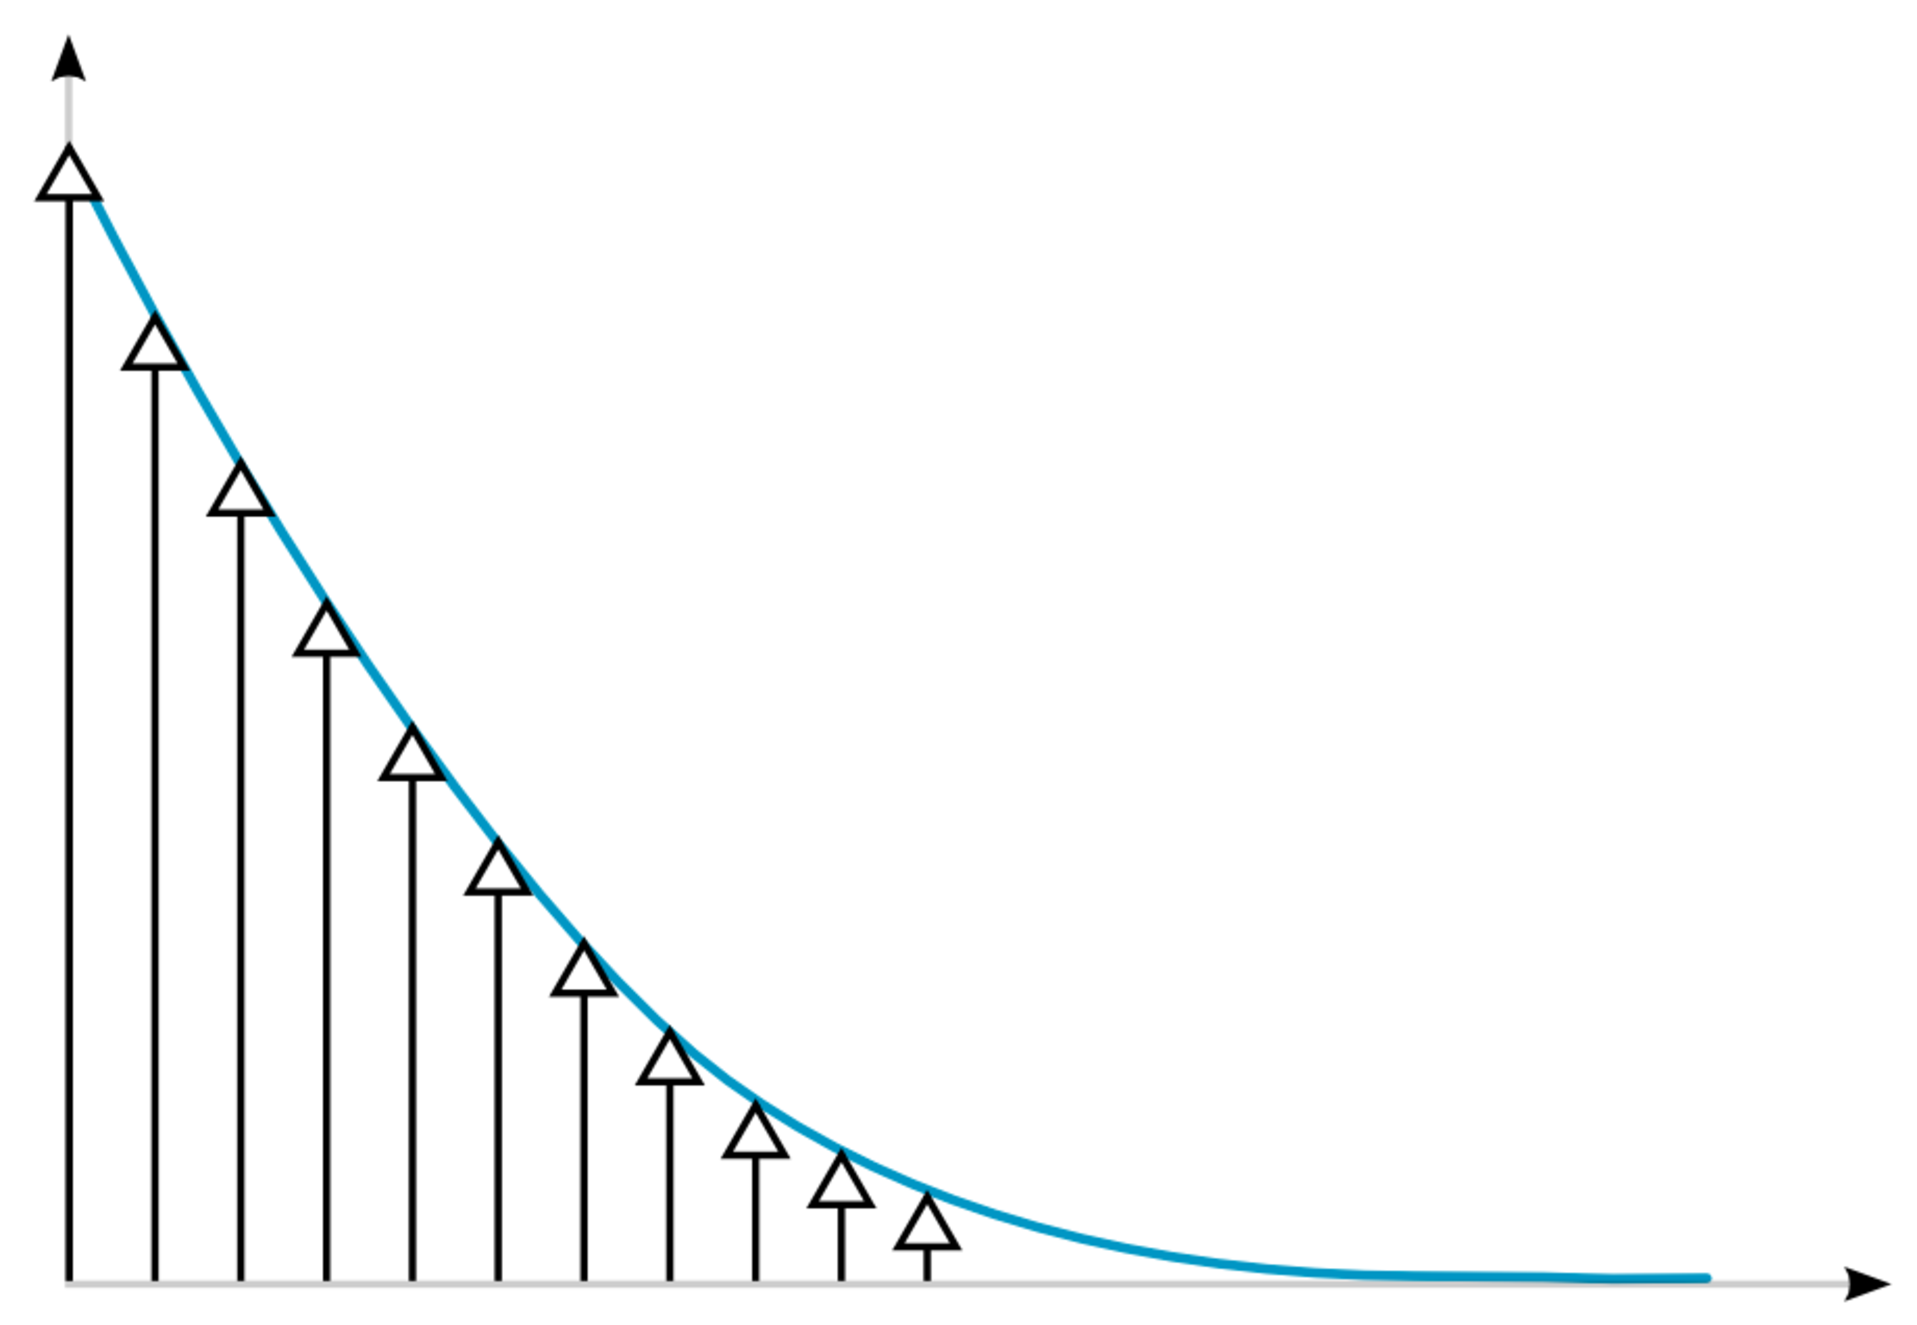
\includegraphics[width=39mm]{momentum_diffusion_profile8.pdf}}
			\put(145, -30){\footnotesize \color{bleu} $v(x, t_3)$}
			\put(118.5, -12){\footnotesize $U_1$}
    \end{picture}
  \end{center}
  \mycaption{Entraînement vertical de fluide par diffusion visqueuse (frottements) horizontale : 
  							évolution de la position des particules fluides (haut) et du profil de vitesse verticale (bas).
							$\delta(t)$ désigne la longueur de pénétration du phénomène.}
  \label{fig:entrainement}
\end{figure}



%==================================================================================================
\section{Méthode}
%==================================================================================================

L'équation (\ref{eq:diffusion}) appartient à la famille des équations linéaires de diffusion 
instationnaire, pour lesquelles il existe plusieurs techniques de résolution mathématique.
Dans le cas présent où il n'y a pas de longueur imposée par le problème (le milieu est semi-infini)
il est possible de rechercher une solution dite \textsl{auto-semblable}, ou \textsl{auto-similaire},
dont la forme générale peut être trouvée
par le biais d'une méthode issue de la théorie des groupes d'invariance des systèmes d'équations.
On se bornera dans cette partie à appliquer cette technique sans la justifier.

\begin{enumerate}
\item
La solution générale peut s'ecrire formellement comme une relation $\mathcal{F}$
entre toutes les variables et paramètres du problème : 
le quintuplet $\{v, x, t, \nu, U_1\}$ est solution de l'équation (\ref{eq:diffusion})
et des conditions limites et initiales associées
si et seulement si $\mathcal{F}(v, x, t, \nu, U_1)=0$.
\\
En appliquant dans l'équation (\ref{eq:diffusion}) et les conditions limites et initiales associées
le changement de variable $v=Av^*$, $x=Bx^*$, $t=Ct^*$, $\nu=D\nu^*$ et $U_1=EU_1^*$,
déterminer les relations que doivent satisfaire les facteurs multiplicatifs 
$A$, $B$, $C$, $D$ et $E$ afin que $\{v^*, x^*, t^*, \nu^*, U_1^*\}$ soit aussi solution.
\item
Les facteurs qui vérifient les deux relations trouvées précédemment décrivent ce que l'on appelle
le groupe d'invariance multiplicatif du système.
Le théorème mathématique sur les groupes d'invariance nous assure que dans ce cas
le quintuplet $\{Av, Bx, Ct, D\nu, EU_1\}$ est aussi solution, c'est-à-dire que
$\mathcal{F}(Av, Bx, Ct, D\nu, EU_1)=0$.
\\
En choisissant $A$, $B$, $C$, $D$ et $E$ de manière judicieuse, montrer que la solution
formelle peut s'écrire $\mathcal{F}(v/U_1, x/\sqrt{\nu t}, 1, 1, 1)=0$, c'est-à-dire 
qu'il existe une relation qui lie $v/U_1$ et $x/\sqrt{\nu t}$, ou encore 
que $v/U_1 = f(x/\sqrt{\nu t})$.
\end{enumerate}

\noindent
En conclusion cette technique mathématique montre que l'on peut chercher une solution de la forme
\begin{equation}
	v(x, t) = U_1\, f(x/\sqrt{\nu t}) = U_1 \, f(\eta),
	\label{eq:similitude}
\end{equation}
où $\eta = x/\sqrt{\nu t}$ est appelée \textsl{variable de similitude} du problème. 

%==================================================================================================
\section{Résolution}
%==================================================================================================

\begin{enumerate}
\item
	Question préliminaire : calculer $\dpdt{\eta}$, $\dpdx{\eta}$ puis $\ddpdx{\eta}$.
\item
	En injectant le changement de variables (\ref{eq:similitude}) dans l'équation (\ref{eq:diffusion}) et dans
	les conditions limites et initiales associées, montrer que le problème à résoudre s'écrit
	\begin{equation}
		f''(\eta) + \frac{1}{2}\eta \, f'(\eta) = 0, \quad \mbox{avec $f(0) = 1$ et $f(\eta\rightarrow \infty) = 0$.}
	\end{equation}
	où le prime $'$ désigne la dérivée par rapport à la variable $\eta$.
\item
	Résoudre l'équation pour $g(\eta) = f'(\eta)$ puis montrer que 
	$
		f(\eta) = 1 - \mbox{erf}\left ( \dfrac{\eta}{2}\right ) = \mbox{erfc}\left ( \dfrac{\eta}{2}\right )
	$
	
	où les fonctions erreur \mbox{erf} et erreur complémentaire \mbox{erfc} sont définies par
	\[
		\mbox{erf}(x) = \frac{2}{\sqrt{\pi}} \, \int_0^x e^{-{x^*}^2}\, dx^*, 
		\quad \mbox{et} \quad \mbox{erfc}(x) = 1 - \mbox{erf}(x).
	\]
	Ces deux fonctions sont tracées sur la figure~\ref{fig:erf}.
	On remarquera que $\mbox{erf}(0) = 0$ et $\mbox{erf}(x\rightarrow +\infty) = 1$.
\item
	En déduire l'expression de la solution $v(x, t)$ et tracer sous Matlab le profil de vitesse adimensionné $v(x, t)/U_1$
	pour différents instants $t$ (on prendra $\nu = 10^{-3}$ m$^2$/s).
\item
	Cette expression fait apparaître la quantité $\delta(t) = \sqrt{\nu t}$ : vérifier qu'il s'agit d'une échelle de longueur.
	Cette échelle caractéristique des problèmes de diffusion est appelée \textsl{longueur ou profondeur de pénétration}, 
	et fournit une \textsl{loi d'échelle} permettant d'estimer la distance sur laquelle le phénomène de diffusion est actif 
	(cf. fig.~\ref{fig:entrainement}).
\item
	Question subsidiaire : déterminer l'expression du frottement pariétal $\myvec{\tau}_p(t)$, 
	c'est-à-dire la contrainte à la paroi.
	On notera $\mu$ la viscosité dynamique du fluide (Pa.s).
\end{enumerate}

\begin{figure}[tbh]
  \begin{center}
    \begin{picture}(60, 38)(-2, 4)
				\put(0, 0){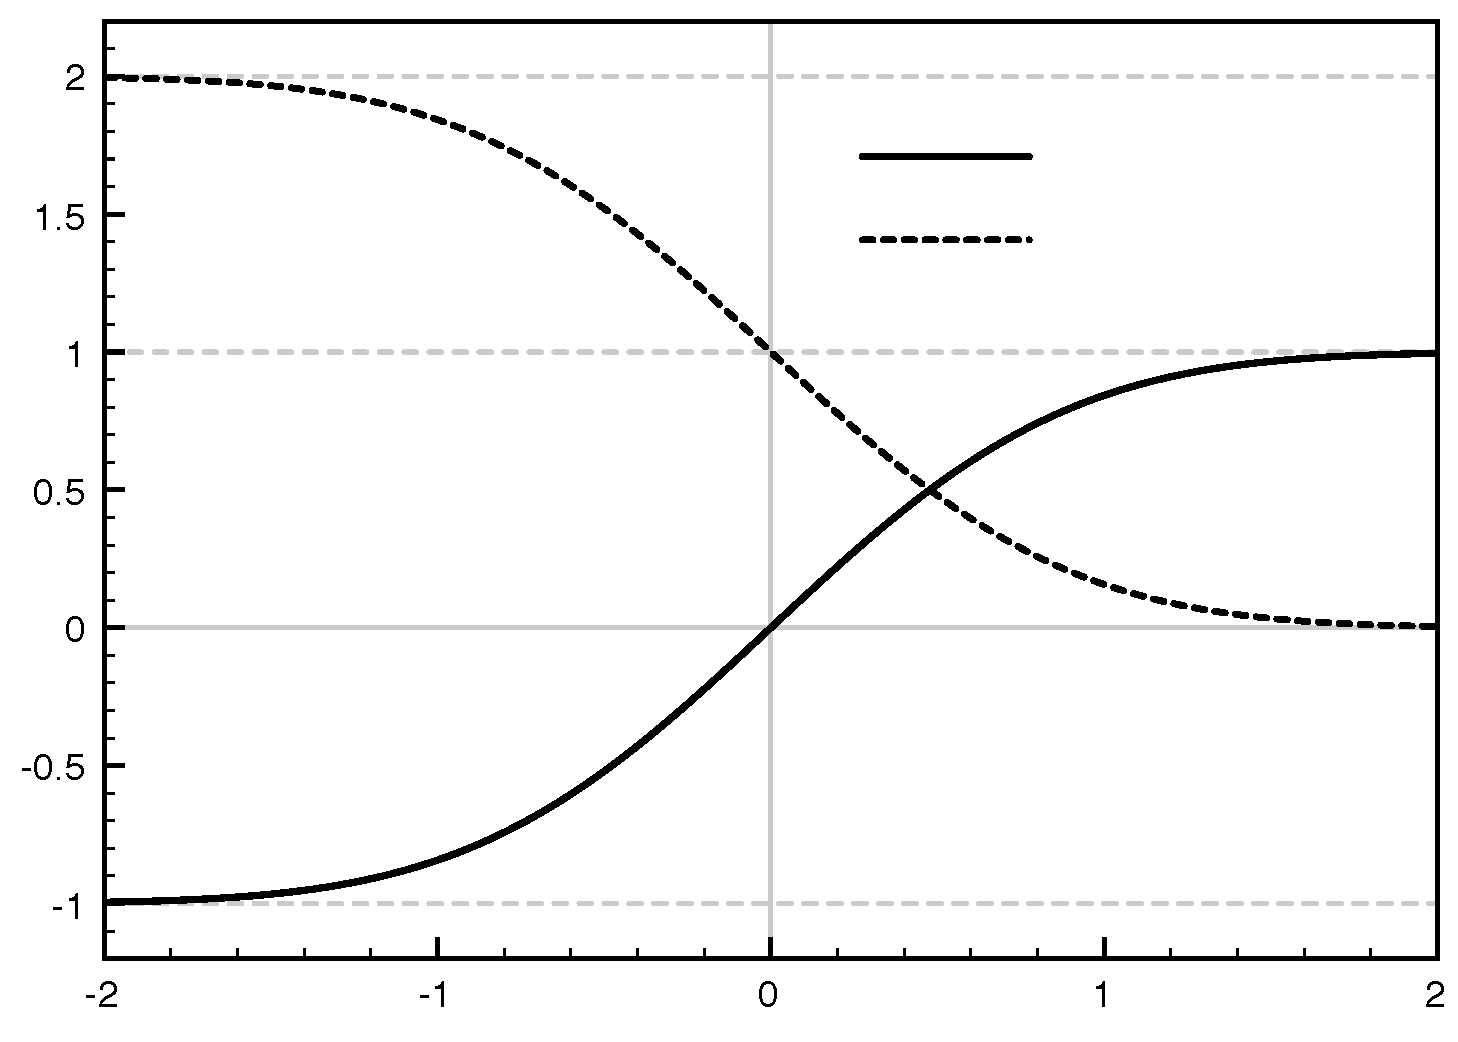
\includegraphics[width=60mm]{erf_erfc.pdf}}
				\put(44, 36){\scriptsize $y=\mbox{erf}(x)$}
				\put(44, 32.5){\scriptsize $y=\mbox{erfc}(x)$}
				\put(31, -2){\scriptsize $x$}
				\put(-2, 16.7){\scriptsize$y$}
     \end{picture}
  \end{center}
  \mycaption{Fonctions erreur {\rm erf} et erreur complémentaire {\rm erfc}.}
  \label{fig:erf}
\end{figure}

%%%%%%%%%%%%%%%%%%%%%%%%%%%%%%%%%%%%%%%%%%%%%%%%%%%%%%%%%%%%%%%%%%%%%%%%%%%%%%%%%%%%%%%%%%%%%%%%%%%
\end{document}
%%%%%%%%%%%%%%%%%%%%%%%%%%%%%%%%%%%%%%%%%%%%%%%%%%%%%%%%%%%%%%%%%%%%%%%%%%%%%%%%%%%%%%%%%%%%%%%%%%%

